\chapter{Introduction to ordinal numbers and ordinal notations}
\label{chap:ON}

The proof of termination of all hydra battles presented in~\cite{KP82} is based
on \emph{ordinal numbers}.
From a mathematical point of view, an ordinal is a representative of an equivalence class for isomorphisms of  totally ordered well-founded sets.

For the computer scientist, ordinals are tools for proving the totality of a given recursive function, or termination of a transition system. \emph{Ordinal arithmetic} 
provides a set of functions whose properties, like \emph{monotony}, allow to define \emph{variants}, \emph{i.e.} strictly decreasing measures used in proofs of termination.

\vspace{4pt}

Let us have a look at Figure~\ref{fig:ordinal-sequence}. It presents a few items of a  sequence of ordinal numbers, which extends the sequence of natural numbers. 




\begin{figure}[h]
  \centering
\fbox{\Large
  \begin{minipage}{1.0\linewidth}
  \begin{align*}
     &\textcolor{blue}{0},\,1,2,3,4,5,6,7,8,9,10,11,12,13,14,15,16,17,\ldots\\
&\textcolor{red}{\omega},\,\omega+1,\omega+2,\omega+3,\ldots\\
&\textcolor{red}{\omega\times 2},\,\omega\times 2+1,\ldots, \textcolor{red}{\omega\times 3},\,\omega\times 3+1,\ldots, \textcolor{red}{\omega\times 4},\ldots\\
&\textcolor{red}{\omega^2},\ldots, \textcolor{red}{\omega^2\times 42},\ldots,\textcolor{red}{\omega^3},\ldots, \textcolor{red}{\omega^4},\omega^4+1,\ldots\\
&\textcolor{red}{\omega^\omega},\ldots, \textcolor{red}{\omega^\omega+\omega^7\times 8},\ldots,\textcolor{red}{\omega^\omega\times 2},\omega^\omega\times 2+1, \ldots\\
&\textcolor{red}{\omega^{\omega^\omega}},\ldots, \textcolor{red}{\omega^{\omega^\omega}+\omega^\omega\times 42+ \omega^{55}+\omega}, \ldots, \textcolor{red}{\omega^{\omega^{\omega+1}}}, \omega^{\omega^{\omega+1}}+1,\dots\\
& \textcolor{red}{\epsilon_0 (= \omega^{\epsilon_0)}}, \epsilon_0+1, \epsilon_0+2, \epsilon_0+3, \ldots\\
& \textcolor{red}{\epsilon_1}, \ldots, \textcolor{red}{\epsilon_2}, \ldots, \textcolor{red}{\epsilon_\omega},\ldots \\
& \textcolor{red}{\Gamma_0}, \Gamma_0+1, \Gamma_0+2, \Gamma_0+3,\ldots, \textcolor{red}{\Gamma_0+\omega}, \ldots\\
&\ldots
  \end{align*}   
  \end{minipage}}
 
 
  \caption{A short overview of the sequence of ordinal numbers}
  \label{fig:ordinal-sequence}
\end{figure}


Let us comment some features of this figure:

\begin{itemize}
\item The ordinals are listed in a strictly increasing order. 
\item Dots : ``$\ldots$'' stand for  infinite sequences of ordinals, not shown for lack of space. For instance, the ordinal $42$ is not shown in the first line, but it exists, somewhere between $17$ and $\omega$.
\item Each ordinal printed in black is the immediate successor of another ordinal. We call it a \emph{successor} ordinal. For instance, $12$ is the successor of $11$, and $\omega^4+1$ the successor of $\omega^4$.
\item Ordinals (displayed in red)  that  follow immediately dots are called \emph{limit ordinals}. With respect to the order induced by this sequence, any limit ordinal $\alpha$ is the least upper bound of  the set $\mathbb{O}_\alpha$ of all ordinals strictly less than $\alpha$.
\item
For instance $\omega$ is the least upper bound of the set of all finite ordinals (in the first line). It is also the first limit ordinal, and the first infinite ordinal, in the sense that 
the set $\mathbb{O}_\omega$ is infinite.
\item The ordinal $\epsilon_0$ is the first number which is equal to its own exponential of base $\omega$. It plays an important role in proof theory, and is particularly studied in chapters~\ref{chap:T1} to \ref{chap:alpha-large}.
\item Any ordinal is  either the ordinal \textcolor{blue}{$0$},
a successor ordinal, or a \textcolor{red}{limit ordinal}.
\end{itemize}




\section{The mathematical point of view}

\subsection{Well-ordered sets}
Let us start with some definitions.
A  \emph{well-ordered set} is a set provided with a binary relation $<$ which has the following properties.
\begin{description}
\item[irreflexivity] : $\forall x\in A, x\not< x$
\item[transitivity] : $\forall x\,y\,z\in A, x<y \Rightarrow y<z \Rightarrow x<z$
\item[trichotomy]: $\forall x\,y\in A, x<y \vee x = y \vee y < x$
\item[well foundedness]: $<$ is well-founded (every element of $A$ is accessible)\footnote{In classical mathematics, we would say that there is no infinite sequence $a_1>a_2> \dots a_n> a_{n+1}\dots$ in $A$. In contrast, \coq's standard library contains
an inductive definition of a predicate \texttt{Acc} which allows us to write 
constructive proofs of accessibility (See \href{https://coq.inria.fr/distrib/current/stdlib/Coq.Init.Wf.html}{Coq.Init.Wf}).}.
\end{description}

The best known examples of well-ordered sets are the set $\mathbb{N}$ of natural numbers (with the usual order $<$), as well as any finite segment $[0,i)=\{j\in\mathbb{N}\,|\,j<i\}$.
The disjoint union of two copies of $\mathbb{N}$, \emph{i.e.} the set $\{0,1\}\times\mathbb{N}$ is also well-ordered,
with respect to the order below:

\begin{align*}
(i,j) < (i,k) & \;\textit{\textbf{if} }\; j < k\\
(0,k) < (1,l) & \;\textit{\textbf{for\,any}}\;k \;\textit{\textbf{and}} \; l
\end{align*}

\subsection{Ordinal numbers}

\index{maths}{Ordinal numbers}

Let $(A,<_A)$ and $(B,<_B)$ two well-ordered sets. $A$ and $B$ are said to have \emph{the same order type} if 
there exists a strictly monotonous bijection $b$ from $A$ to $B$, \emph{i.e.} which verifies the proposition
$\forall x\,y\in A,\, x <_A y \Rightarrow b(x) <_B  b(y)$.

Having the same order type is an equivalence relation between well-ordered sets. Ordinal numbers (in short: \emph{ordinals})  are descriptions (\emph{names}) of the equivalence classes.
For instance, the order type of $(\mathbb{N},<)$ is associated with the ordinal called  $\omega$, and the order we considered on 
the disjoint union of $\mathbb{N}$ and itself is named $\omega+\omega$.

In a set-theoretic framework, one can consider any ordinal $\alpha$ as a well-ordered set, whose  elements are just the ordinals strictly less than $\alpha$, \emph{i.e.} the \emph{segment} $\mathbb{O}_\alpha=[0, \alpha)$. So, one can speak about \emph{finite}, \emph{infinite}, \emph{countable}, etc., ordinals. Nevertheless, since we work within type theory, 
we do not identify ordinals as sets of ordinals, but consider the correspondence between ordinals and sets of ordinals as the function that maps $\alpha$ to $\mathbb{O}_\alpha$.
For instance $\mathbb{O}_\omega=\mathbb{N}$, and $\mathbb{O}_7=\{0,1,2,3,4,5,6\}$.


We cannot cite all the literature published on ordinals since Cantor's book
\cite{cantorbook}, and 
leave it to the reader to explore the bibliography.

The introduction of Jos\'e Grimm's report~\cite{grimm:hal-00911710} contains a nice presentation of the main properties of ordinals.


\section{Ordinal numbers in Coq}

Two kinds of representation of ordinals are defined in our development.

\begin{itemize}
\item A ``mathematical'' representation of the set of countable ordinal numbers, after Kurt Schütte~\cite{schutte}. This representation uses several (hopefully harmless) axioms. We use it as a reference for proving the correctness of ordinal notations.

  \index{gaiabridge}{Introduction}
  \gaiasign
  We are also progressively importing \gaia's~\cite{Gaia} definitions and theorems, based on Bourbaki's set theory~\cite{Grimm2016}. Chapter~\ref{gaia-chapter} is dedicated to the connexion between libraries \HydrasLib and \gaia.
  
\item A family of \emph{ordinal notations} (also called \emph{[ordinal] notation systems}), \emph{i.e.} data types used to represent segments $[0,\mu)$, where $\mu$ is some countable ordinal. Each ordinal notation is defined inside the Calculus of Inductive Constructions (without axioms). Many functions are defined, allowing proofs by computation. Note that proofs of 
correctness of a given ordinal notation with respect to Schütte's model obviously use axioms.
Please execute the \texttt{Print Assumptions} command in case of doubt.
\end{itemize}

% \section{Countable ordinals}

% Chapter~\ref{chap:schutte} of this document presents an adaptation to \coq{} of an axiomatization in classical logic of the set of countable ordinals by K. Schütte~\cite{schutte}. 
% That formalization is quite complex, technical and unshamedly non-constructive,  so we put its description  in the last chapter of this document. 

% Please note that Schütte considers the (uncountable) set $\mathbb{O}$ of all countable ordinals. This set is well ordered (which is one of Schütte's axioms), and associates to any ordinal $\alpha$ the segment $\mathbb{O}_\alpha$ of all ordinals strictly less than $\alpha$.

% In our adaptation to \coq{}, we declare a type \texttt{Ord}, a binary relation \texttt{lt} (with infix notation \texttt{"\_<\_"}, and assume Schütte's axiom. In Chapter~\ref{chap:schutte},
% we derive some interesting properties of countable ordinals from these axioms.

It is interesting to compare proofs of a given property (for instance the associativity of addition) both in the computational framework of some ordinal notation, and in mathematical  models
of Schütte or \gaia.

\section{Ordinal Notations}


Fortunately, the ordinals we need for  studying hydra battles are much simpler than Schütte's, and can be represented as quite simple data types in \gallina. 

Let $\alpha$ be some (countable) ordinal; 
in \coq{} terms, we call \emph{ordinal notation for $\alpha$} a structure composed 
of:
\begin{itemize}
\item A data type $A$ for representing all ordinals strictly below $\alpha$,
\item A well founded order $<$ on $A$, 
\item A correct function for comparing two ordinals. Note  that the reflexive closure of $<$ is thus a \emph{total order}.
\end{itemize}


Such a structure may be proved correct relatively to a bigger ordinal notation or to Schütte's or \gaia's model.





\subsection{Classes for ordinal notations}

From the \coq{} user's point of view, an ordinal notation is
a structure allowing to compare two ordinals by computation, and proving by well-founded induction.

\subsubsection{The \texttt{Comparison} and \texttt{Comparable} classes}

We use the operational class \texttt{Comparison} of comparison functions to define the \texttt{Comparable} class, contributed by Jérémy Damour and Théo Zimmermann, which allows us to apply generic lemmas and tactics about decidable strict orders.
The correctness of the comparison function is expressed through Stdlib's type 
\texttt{Datatypes.CompareSpec} as specialized by \texttt{Datatypes.CompSpec}.

\begin{Coqsrc}
  Inductive CompareSpec (Peq Plt Pgt : Prop) :
  comparison -> Prop :=
    CompEq : Peq -> CompareSpec Peq Plt Pgt Eq
  | CompLt : Plt -> CompareSpec Peq Plt Pgt Lt
  | CompGt : Pgt -> CompareSpec Peq Plt Pgt Gt.

Definition CompSpec {A} (eq lt : A -> A -> Prop) (x y : A) :=
 CompareSpec (eq x y) (lt x y) (lt y x).
\end{Coqsrc}

\emph{From Module~\href{../theories/html/hydras.Prelude/mparable.html\#Hvariant}{Prelude.Comparable}}

\label{sect:comparable-def}

\input{movies/snippets/Comparable/ComparableDef}





\subsubsection{The \texttt{ON} class}

The following class definition, parameterized with a type $A$, a binary relation \texttt{lt} on $A$, specifies that \texttt{lt} is a well-founded strict order, provided with a correct comparison function.


\vspace{4pt}
\noindent\emph{From
Library~\href{../theories/html/hydras.OrdinalNotations.ON_Generic.html}{OrdinalNotations.ON\_Generic}}

\label{types:ON}
\index{hydras}{Library OrdinalNotations!Type classes!ON}

\begin{alectryon}
  % Generator: Alectryon
  \sep
  \begin{sentence}
    \begin{input}
      \PY{k+kn}{Class}~\PY{n+nf}{ON}~\PY{o}{\PYZob{}}\PY{n+nv}{A}\PY{o}{:}\PY{k+kt}{Type}\PY{o}{\PYZcb{}}~\PY{o}{(}\PY{n+nv}{lt}\PY{o}{:}~\PY{n}{relation}~\PY{n}{A}\PY{o}{)}~\PY{o}{(}\PY{n+nv}{cmp}\PY{o}{:}~\PY{n}{Compare}~\PY{n}{A}\PY{o}{)}~\PY{o}{:=}\nl
      ~~\PY{o}{\PYZob{}}\nl
      ~~\PY{n}{ON\PYZus{}comp}~\PY{o}{:\PYZgt{}}~\PY{n}{Comparable}~\PY{n}{lt}~\PY{n}{cmp}\PY{o}{;}\nl
      ~~\PY{n}{ON\PYZus{}wf}~\PY{o}{:}~\PY{n}{well\PYZus{}founded}~\PY{n}{lt}\PY{o}{;}\nl
      ~~\PY{o}{\PYZcb{}.}
    \end{input}
  \end{sentence}
\end{alectryon}


We give  also a few handy definitions and lemmas for any ordinal notation.

\label{sect:on-lt-notation}
\label{sect:on-le-notation}
\label{sect:measure-ON}
\label{sect:bigO-ON}


\inputsnippets{ON_Generic/ONDefsa}
\inputsnippets{ON_Generic/ONDefsb}

\begin{remark}
The infix notations \texttt{o<} and \texttt{o<=} are defined in order to make apparent the distinction between the various notation scopes that may co-exist in a same statement. So the infix \texttt{<} and \texttt{<=} are reserved to the natural numbers. In the mathematical formulas, however, we still use $<$ and $\leq$ for comparing ordinals.
\end{remark}


% \subsection{Ordinal notations and  termination measures}
% \label{sect:measure-ON}

% The following lemma (together with the type class mechnism) allows us to define termination measures over any ordinal notation. It is just an application of  the libraries \texttt{Coq.Wellfounded.Inverse\_Image}
% and  \texttt{Coq.Wellfounded.Inclusion}. 

% \begin{Coqsrc}
% Definition measure_lt {A:Type}{lt: relation A}
%             {compare : A -> A -> comparison}
%             {on : ON lt compare}
%             {B : Type} (m : B -> A) : relation B :=
%              fun x y => on_lt (m x) (m y).
            
% Lemma wf_measure  {A:Type}(lt: relation A)
%             {compare : A -> A -> comparison}
%             {on : ON lt compare}
%             {B : Type}
%             (m : B -> A):  well_founded (measure_lt m). 
% \end{Coqsrc}

% A simple example of application is given in Sect.~\vref{sect:merge-example}.


\section{Example: the ordinal \texorpdfstring{$\omega$}{omega}}




The simplest example of ordinal notation is built over the type \texttt{nat} of \coq's standard library. We just have to apply already proven lemmas about Peano numbers.

\vspace{4pt}
\noindent\emph{From Library~\href{../theories/html/hydras.OrdinalNotations.ON_Omega.html}{OrdinalNotations.ON\_Omega}}

\inputsnippets{ON_Omega/OmegaDefa, ON_Omega/OmegaDefb}


\section{Sum of  two ordinal notations}

Let \texttt{NA} and \texttt{NB} be two ordinal notations, on the respective types \texttt{A} and \texttt{B}.

 We consider a new strict order
on the disjoint sum of the associated types, by putting all elements of \texttt{A} before the elements of \texttt{B} (thanks to Standard Library's relation operator \texttt{le\_AsB}).

\vspace{4pt}
\noindent
\emph{From Library~\href{https://coq.inria.fr/distrib/current/stdlib/Coq.Relations.Relation_Operators.html}{Relations.Relation\_Operators}}.

\begin{Coqanswer}
Inductive
le_AsB (A B : Type) (leA : A -> A -> Prop) (leB : B -> B -> Prop)
  : A + B -> A + B -> Prop :=
| le_aa : forall x y : A, leA x y -> le_AsB A B leA leB (inl x) (inl y)
| le_ab : forall (x : A) (y : B), le_AsB A B leA leB (inl x) (inr y)
| le_bb : forall x y : B, leB x y -> le_AsB A B leA leB (inr x) (inr y)
\end{Coqanswer}

%\pagebreak

\vspace{4pt}
\noindent\emph{From Library~\href{../theories/html/hydras.OrdinalNotations.ON_plus.html}{OrdinalNotations.ON\_plus}}


\input{movies/snippets/ON_plus/Defs}

In order to build an instance of \texttt{Comparable}, we have to define a correct comparison function.

\inputsnippets{ON_plus/compareDef, ON_plus/compareCorrect}
\inputsnippets{ON_plus/plusComp}


Standard library's lemma \texttt{Wellfounded.Disjoint\_Union.wf\_disjoint\_sum} 
is applied  to prove that our order \texttt{lt} is well-founded, allowing us to build an instance of \texttt{ON}:

\inputsnippets{ON_plus/ltWf, ON_plus/OnPlus}

\subsection{The ordinal \texorpdfstring{$\omega+\omega$}{omega + omega}}

The ordinal $\omega+\omega$ (also known as $\omega\times 2$) may be represented as the concatenation 
of two copies of $\omega$ (Figure~\ref{fig:omega-plus-omega}).
It is also represented by the two first lines of Figure~\ref{fig:ordinal-sequence}.

\begin{figure}[h]
   \centering
   \begin{tikzpicture}[very thick, scale=0.5]
\begin{scope}[color=blue]
\node(A0) at (2,0)[label=below:$0$]{$\bullet$};
\node(A1) at (3,0)[label=below:$1$]{$\bullet$};
\node(A2) at (4,0)[label=below:$2$]{$\bullet$};
\node (Adots) at (6,0) {$\ldots$};
\node(An) at (8,0)[label=below:$n$]{$\bullet$};
\node(A2) at (10,0)[label=below:$n+1$]{$\bullet$};
\node (Adots1) at (12,0) {$\ldots$};
\end{scope}
\begin{scope}[color=red]
\node(B0) at (14,0)[label=below:$0$,label=above:\textcolor{red}{$\omega$}]{$\bullet$};
\node(B1) at (16,0)[label=below:$1$, label=above:$\omega+1$]{$\bullet$};
\node(B2) at (18,0)[label=below:$2$,label=above:$\omega+2$]{$\bullet$};
\node (Bdots) at (20,0) {$\ldots$};
\node (Bn) at (22,0) [label=below:$p$, label=above:$\omega+p$]{$\bullet$};
\node (Bdots2) at (24,0) {$\ldots$};
\end{scope}
\end{tikzpicture}
   \caption{\textcolor{blue}{$\omega+{\color{red}\omega}$}}
   \label{fig:omega-plus-omega}
 \end{figure}

We can define this notation in \coq{} as an instance of \texttt{ON\_plus}.


\vspace{4pt}
\noindent\emph{From Module~\href{../theories/html/hydras.OrdinalNotations.ON_Omega_plus_omega.html}{OrdinalNotations.ON\_Omega\_plus\_omega}}

\input{movies/snippets/ON_Omega_plus_omega/OmegaPlusOmegaDef}

\vspace{4pt}

We can now define abbreviations. For instance, the finite ordinals are represented by terms built with  the constructor \texttt{inl}, and the first infinite ordinal $\omega$ by the term \texttt{(inr 0)}.

\vspace{4pt}

\input{movies/snippets/ON_Omega_plus_omega/finiteOmega}

\vspace{4pt}

\input{movies/snippets/ON_Omega_plus_omega/ltOmega}



% \label{warning:coercions}
% \index{Coq!Coercions} 
% \begin{remark}
% Beware of coercions and notation scopes!
% Let us consider the following goal:

% \begin{Coqsrc}
%  Goal (6 o< 8).
%  auto with arith.
% \end{Coqsrc}


% \begin{Coqanswer}
% 1 subgoal (ID 9)
  
%   ============================
%   6 o< 8
% \end{Coqanswer}

% Please keep in mind that the current notation scope interprets the infix \texttt{``<''} as the predicate \texttt{Omega\_plus\_omega.lt} and not \texttt{Nat.lt}. More,  the coercion mechanism converts the terms \texttt{6:nat} [resp. \texttt{8:nat} ]
% into \texttt{inl 6} [resp. \texttt{inl 8}].  So, the initial goal is correctly interpreted by \coq{}, but not as an inequality between two natural numbers.


% \begin{Coqsrc}
% Set Printing All.
% \end{Coqsrc}

% \begin{Coqanswer}
% 1 subgoal (ID 337)
  
%   ============================
%   @on_lt nat Peano.lt Nat.compare Omega (S (S (S (S (S (S O))))))
%     (S (S (S (S (S (S (S (S O))))))))
% \end{Coqanswer}


% Anyway, the initial goal is provable, using \texttt{le\_AsB}'s first constructor.

% \begin{Coqsrc}
%   constructor; auto with arith.
% Qed.
% \end{Coqsrc}

% \end{remark}
%



\section{Limits and successors}

Let us look again at our implementation of $\omega+\omega$. We can classify its elements into three categories:

\begin{itemize}
\item The least ordinal, \texttt{(inl 0)}, also known as  \texttt{(fin 0)}.
\item The first infinite ordinal $\omega$.
\item The remaining ordinals, either of the form \texttt{(inl (S $i$))} or \texttt{(inr (S $i$))} (in black on Figure~\ref{fig:ordinal-sequence}), called \emph{successor ordinals}.
\end{itemize}

\subsection{Definitions}
It would be interesting to specify at the most generic level, what is a zero, a successor or a limit ordinal. Let $<$ be a strict order on a type $A$.

\begin{itemize}
\item A \emph{least} element is a minorant (in the large sense) of the full set  on $A$,
\item $y$ is a \emph{successor} of $x$ if $x<y$ and there is no element between $x$ and $y$. We will also say that $x$ is a \emph{predecessor} of $y$.
\item $x$ is a \emph{limit} if $x$ is not a least element, and for any $y$ such that $yo<x$,
 there exists some $z$ such that $y<z<x$.
\end{itemize}


The following definitions are in Library \href{../theories/html/hydras.Prelude.MoreOrders.html}{Prelude.MoreOrders}.

\input{movies/snippets/MoreOrders/Defs}


\index{hydras}{Exercises}
\begin{exercise}
Prove, that, in any ordinal notation system, every ordinal has at most one predecessor, and at most one successor. 

\emph{You may start this exercise with the file
\href{https://github.com/coq-community/hydra-battles/blob/master/exercises/ordinals/predSuccUnicity.v}{exercises/ordinals/predSuccUnicity.v}.}

\end{exercise}

\index{hydras}{Exercises}
\begin{exercise}
Prove, that, in any ordinal notation system, if $\beta$ is a successor of $\alpha$,
then for any $\gamma$, $\gamma<\beta$ implies 
$\gamma\leq\alpha$.

\emph{You may start this exercise with the file
\href{https://github.com/coq-community/hydra-battles/blob/master/exercises/ordinals/lt_succ_le.v}{exercises/ordinals/lt\_succ\_le.v}.}
\end{exercise}




\subsection{Limits and successors in \texorpdfstring{$\omega+\omega$}{omega+omega}}

Using the definitions above, we can prove the following lemma:

\vspace{4pt}

\noindent\emph{From Module~\href{../theories/html/hydras.OrdinalNotations.ON_Omega_plus_omega.html}{OrdinalNotations.ON\_Omega\_plus\_omega}}

\input{movies/snippets/ON_Omega_plus_omega/limitIff}

\vspace{4pt}

Regarding successors, let us define the following function and prove its correctness:


\input{movies/snippets/ON_Omega_plus_omega/succDef}

\input{movies/snippets/ON_Omega_plus_omega/succCorrect}

\vspace{4pt}



We can also check whether an ordinal is a successor by a simple computation:

\input{movies/snippets/ON_Omega_plus_omega/succb}

\vspace{4pt}

Finally, the nature of any ordinal is decidable (inside this notation system) :



\noindent\emph{From Module~\href{../theories/html/hydras.OrdinalNotations.ON_Omega_plus_omega.html}{OrdinalNotations.ON\_Omega\_plus\_omega}}

\input{movies/snippets/ON_Omega_plus_omega/ZeroLimitSuccDec}

\section{Product of ordinal notations}

Let \texttt{NA} and \texttt{NB} be two ordinal notations, on the respective  ordered types \texttt{A} and \texttt{B}. The product of \texttt{NA} and \texttt{NB} is considered as the concatenation of $B$ copies of $A$, ordered by the lexicographic order on $B\times A$.

In \coq{}, we build an instance of class \texttt{ON} through a sequence of steps as for the sum of ordinal notations.

\vspace{4pt}
\noindent
\emph{From Module~\href{../theories/html/hydras.OrdinalNotations.ON_mult.html}{OrdinalNotations.ON\_mult}}

\inputsnippets{ON_mult/Defs}
\inputsnippets{ON_mult/multComp,  ON_mult/ONMult}
\inputsnippets{ON_mult/endDefs} 

\section{The ordinal \texorpdfstring{$\omega^2$}{omega2}}

The ordinal $\omega^2$ (also called $\phi_0(2)$, see Chap.~\ref{chap:schutte}), is an instance of the multiplication presented in the preceding section.

\vspace{4pt}
\noindent\emph{From Module~\href{../theories/html/hydras.OrdinalNotations.ON_Omega2.html}{OrdinalNotations.ON\_Omega2}}

\inputsnippets{ON_Omega2/Omega2Def, ON_Omega2/Defs}
\inputsnippets{ON_Omega2/Ex1}

\subsection{Arithmetic of \texorpdfstring{$\omega^2$}{omega^2}} 

\subsubsection{Successor}

The successor of any ordinal is defined by a simple pattern-matching.

\input{movies/snippets/ON_Omega2/succ}


This function is proved to be correct w.r.t. the \texttt{Successor} predicate.

\input{movies/snippets/ON_Omega2/succOK}

\input{movies/snippets/ON_Omega2/succLemmas}


\subsubsection{Addition}

We can define on \texttt{Omega2} an addition which extends the addition on \texttt{nat}. Please note that this operation is not commutative:

\inputsnippets{ON_Omega2/plusDef, ON_Omega2/plusExamples}


\subsubsection{Multiplication}

The restriction of ordinal multiplication to the segment $[0,\omega^2)$ is not a total function.
For instance $\omega\times\omega= \omega^2$ is outside the set of represented values.
Nevertheless, we can define two operations mixing natural numbers and ordinals.

\input{movies/snippets/ON_Omega2/multFinDef}
\input{movies/snippets/ON_Omega2/multFinExamples}


Multiplication with a finite ordinal and addition are related through the following lemma:

 
\inputsnippets{ON_Omega2/uniqueDecompositiona,
  ON_Omega2/uniqueDecompositionb,
  ON_Omega2/uniqueDecompositionz}

\subsection{A proof of termination using \texorpdfstring{$\omega^2$}{omega^2}} 
\label{sect:merge-example}

Using the lemma of Sect.~\vref{sect:measure-ON}, we can define easily a total function which merges two lists (example contributed by Pascal Manoury).

%\index{coq}{Commands!Function}

\vspace{4pt}
\noindent\emph{From Module~\href{../theories/html/hydras.OrdinalNotations.ON_Omega2.html}{OrdinalNotations.ON\_Omega2}}


\inputsnippets{ON_Omega2/Merge, ON_Omega2/Mergeb}
 

\subsection{Yet another  proof of impossibility}
\label{omega2-case}

In Sect.~\vref{omega-case}, we proved that there exists no variant from \texttt{Hydra} to \texttt{(nat,$<$)}
(\emph{i.e.} the ordinal $\omega$) for proving the termination of all hydra battles.
We  prove now that  the ordinal $\omega^2$ is also insufficient for this purpose. 

The proof we are going to comment has exactly the same structure as in Section~\ref{omega-case}.
 Nevertheless, the proof of technical  lemmas is a little more complex, due to 
 the structure of the lexicographic order on $\mathbb{N}\times\mathbb{N}$. 
Consider for instance that there exists an infinite number of ordinals  between
$\omega$ and $\omega\times 2$.



The detailed  proof script is in the file
\href{https://github.com/coq-community/hydra-battles/blob/master/theories/ordinals/Hydra/Omega2_Small.v}{theories/ordinals/Hydra/Omega2\_Small.v}.

\subsubsection{Preliminaries}
Let us assume there is a variant from \texttt{Hydra} into $\omega^2$  for proving the   termination of all hydra battles.

\vspace{4pt}
\emph{From Module~\href{../theories/html/hydras.Hydra.Omega2_Small.html}{Hydra.Omega2\_Small}}

\input{movies/snippets/Omega2_Small/Impossibility}
\input{movies/snippets/Omega2_Small/Impossibilitya}



We  follow the same pattern as in Sect.~\ref{omega-case}.
First, we define an injection $\iota$ from type \texttt{ON\_Omega2.t} into \texttt{Hydra}, by
 associating to  each ordinal $\omega\times i+ j = (i,j)$ the hydra with $i$ branches of length $2$ and
$j$ branches of length $1$.

%% revenir ici

\vspace{4pt}
\emph{From Module ~\href{../theories/html/hydras.Hydra.Omega2_Small.html\#iota}{Hydra.Omega2\_Small}}


\input{movies/snippets/Omega2_Small/Impossibilityc}

For instance, Figure~\vref{fig:essai2} shows the hydra associated to the ordinal 
$(3,5)$, a.k.a. $\omega\times 3 + 5$.

\begin{figure}[htb]
\centering
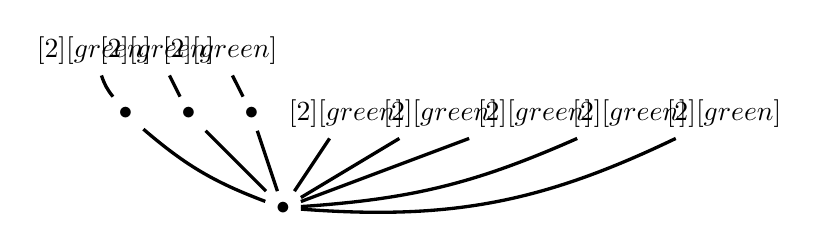
\begin{tikzpicture}[very thick, scale=0.4]
\node (foot) at (6,0) {$\bullet$};
\node (N1) at (1,3) {$\bullet$};
\node (N2) at (3,3) {$\bullet$};
\node (N3) at (5,3) {$\bullet$};
\node (N4) at (8,3) {$\Smiley[2][green]$};
\node (N5) at (11,3) {$\Smiley[2][green]$};
\node (N6) at (14,3) {$\Smiley[2][green]$};
\node (N7) at (17,3){$\Smiley[2][green]$};
\node (N8) at (20,3){$\Smiley[2][green]$};
\node  (N9) at (0,5) {$\Smiley[2][green]$};
\node (N10) at (2,5) {$\Smiley[2][green]$};
\node (N11) at (4,5) {$\Smiley[2][green]$};
\draw (foot) to [bend left=10] (N1);
\draw (foot) -- (N2);
\draw (foot) -- (N3);
\draw (foot) -- (N4);
\draw (foot) -- (N5);
\draw (foot) -- (N6);
\draw (foot) to [bend right=10] (N7);
\draw (foot) to [bend right=15] (N8);
\draw (N1) to [bend left=10] (N9);
\draw (N2) -- (N10);
\draw (N3) -- (N11);
\end{tikzpicture}
\caption{\label{fig:essai2}
The hydra $\iota(\omega\times 3+5)$}
\end{figure}




Like in Sect.~\ref{omega-case}, we build a hydra out of the range of \texttt{iota} (represented in Fig.~\vref{fig:h-omega2-small}).

\begin{figure}[htb]
\centering
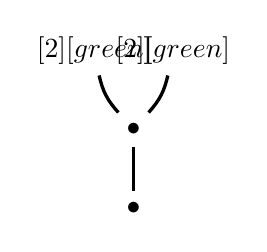
\begin{tikzpicture}[very thick, scale=0.5]
\node (foot) at (2,0) {$\bullet$};
\node (N1) at (2,2) {$\bullet$};
\node (N2) at (3,4) {$\Smiley[2][green]$};
\node (N3) at (1,4) {$\Smiley[2][green]$};
\draw (foot) -- (N1);
\draw (N1) to [bend right =15] (N2);
\draw (N1) to  [bend left=15](N3);
\end{tikzpicture}
\caption{\label{fig:h-omega2-small}}
 The hydra \texttt{big\_h}.
\end{figure}


\input{movies/snippets/Omega2_Small/Impossibilityb}

 
 In a second step, we build a ``smaller'' hydra\footnote{With respect to the measure $m$.}.
 
\input{movies/snippets/Omega2_Small/Impossibilityd}

\vspace{4pt}

Like in Sect.~\ref{omega-case}, we prove the inequality $m\;\texttt{big\_h} \,\texttt{o<=}\, m\;\texttt{small\_h} \,\texttt{o<=}\, m\;\texttt{big\_h}$, which is obviously false.

\subsubsection{Proof of the inequality \texttt{m small\_h o< m big\_h}}

In order to prove the inequality  \texttt{m\_lt: m small\_h o< m big\_h}, it suffices to
build a battle transforming \texttt{big\_h} into \texttt{small\_h}.

First we prove that \texttt{small\_h} is reachable from \texttt{big\_h} in one or two steps. Let us decompose \texttt{m big\_h} as $(i,j)$.
If $j=0$, then one round suffices to transform \texttt{big\_h} into $\iota(i,j)$.
If $j>0$, then a first round transforms \texttt{big\_h} into $\iota(i+1,0)$ and a second round into $\iota(i,j)$. So, we have the following result.

\input{movies/snippets/Omega2_Small/bigToSmall}

Since $m$ is a variant, we infer the following inequality:

\input{movies/snippets/Omega2_Small/mLt}



\subsubsection{Proof of the inequality \texttt{m big\_h o<= m small\_h} }


The proof of the inequality \texttt{m big\_h o<= m small\_h} is quite more complex than in Sect~\ref{omega-case}.  If we consider any ordinal $\alpha=(i,j)$, where $i>0$, there exists an infinite number of
ordinals strictly less than $\alpha$, and there exists an infinite number of battles that start from
$\iota(\alpha)$. Indeed, at any configuration $\iota(k,0)$, where $k>0$, the hydra can freely choose any replication number. Intuitively, the measure of such a hydra must be large enough for taking into account
all the possible battles issued from that hydra.
Let us now give more technical details.

The first steps of our proof start a well-founded induction over $\omega^2$.


\input{movies/snippets/Omega2_Small/mGe}


A case analysis on $i$ and $j$ allows us to
consider three cases :

\begin{itemize}
\item $i=j=0$: the inequality is trivial.
\item $i=1+l, j=0$ ($(i,j)$ is a limit ordinal): By the induction hypothesis \texttt{IHij},
  $(l,k)\texttt{o<=} m(\iota(l,k))$ for any $k$. But (by the rules of the hydra game), $\iota(i,0)$ is transformed into any $\iota(l,k)$ in one round. Thus $m(\iota(l,k)) < m(\iota(i,0))$ for any $k$.
  Therefore, $(l,k) <  m(\iota(i,0))$ for any $k$, thus
  $(i,0)\,\texttt{o<=}\,m(\iota(i,0))$.
 \item $j= l+1$  ($(i,j)$ is a successor). We apply the induction hypothesis to the pair $(i,l)$.
 \end{itemize}

 Please look at the proof script for more details.
 
 \input{movies/snippets/Omega2_Small/mGeb}

\subsubsection{End of the proof}
From \texttt{m\_ge}, we get \texttt{$m$\, big\_h o<= $m$\, small\_h = $m$\,(iota (m big\_h)) }. 
Since $<$ is a strict order (irreflexive  and transitive), this inequality is incompatible with the strict inequality  \texttt{m small\_h o< m big\_h} (lemma \texttt{m\_lt}).


\vspace{4pt}
\noindent
\emph{From Module~\href{../theories/html/hydras.Hydra.Omega2_Small.html\#Impossible}{Hydra.Omega2\_Small}}


  \input{movies/snippets/Omega2_Small/Impossible}

\index{hydras}{Exercises}

\begin{exercise}
Prove that there exists no variant $m$ from \texttt{Hydra} into $\omega^2$ for proving
    the  termination of all \emph{standard} battles.
\end{exercise}



\begin{remark}
 We  prove in Chapter~\ref{ks-chapter} a generalization of the impossibility lemmas of
Sect.~\ref{omega-case} and this section, with the same proof structure, but with much more 
complex technical details.
 \end{remark}

% \index{Exercises}
% \begin{exercise}

% \label{sec:orgheadline63}
% Write \emph{direct} proofs ({i.e.},  without applying the result and tools of Chap.~\ref{ks-chapter}) that the following data structures  are too simple for defining a variant for any hydra battle.

% \begin{itemize}
% \item  $\omega^n$ : the set of all $n$-uples of natural numbers, ordered  by 
%   lexicographic ordering
% \item  $\omega^\omega$: the set of all decreasing sequences (with respect to $\le$)  of natural numbers, ordered by lexicographic ordering on lists.

% For instance, the following inequality holds:
% \[\langle 4,3,3,3,3,3,3,2,2,2 \rangle\,<\,\langle 4,4,2 \rangle\]
% \end{itemize}

  
% \end{exercise}


\section{A notation for finite ordinals}


Let $n$ be some natural number. The segment associated with $n$ is the interval 
$[0,n)\,=\,\{0,1,\dots,n-1\}$. 
One may represent the ordinal $n$ by a sigma type.


\vspace{4pt}
\noindent\emph{From Module~\href{../theories/html/hydras.OrdinalNotations.ON_Finite.html}{OrdinalNotations.ON\_Finite}}

\label{def:Finite-ord-type}

\input{movies/snippets/ON_Finite/Defs}

\subsubsection{Examples}

For instance, let us build two elements of the segment $[0, 7)$, \emph{i.e.} two
inhabitants of   type (\texttt{t 7}), and prove a simple  inequality (see Fig.~\ref{fig:O7}).

\begin{figure}[h]
\centering
\begin{tikzpicture}[very thick, scale=0.6]

\node (N0) at (0,0) {$\bullet$};
\node (i0) at (0,1) {$0$};
\node (N1) at (2,0) {$\bullet$};
\node (i1) at (2,1) {$1$};
\node (N2) at (4,0) {$\bullet$};
\node (i2) at (4,1) {$2$};
\node (N3) at (6,0) {$\bullet$};
\node (i3) at (6,1) {$3$};
\node (N4) at (8,0) {$\bullet$};
\node (i4) at (8,1) {$4$};
\node (N5) at (10,0) {$\bullet$};
\node (i5) at (10,1) {$5$};
\node (N6) at (12,0) {$\bullet$};
\node (i6) at (12,1) {$6$};
\node(alpha1) at (4,-1) {$\alpha_1$};
\node(alpha2) at (10,-1) {$\beta_1$};
\end{tikzpicture}

\caption{The segment $\mathbb{O}_7$\label{fig:O7}}
\end{figure}
  
%\index{coq}{Commands!Program}

\input{movies/snippets/ON_Finite/Example1}




Note that the type (\texttt{t 0}) is empty, and that, for any natural number
 $n$, $n$ does not belong to (\texttt{t $n$}).

 \inputsnippets{ON_Finite/t0Empty, ON_Finite/bad10}

\subsubsection{Comparison function}

In order to build an instance of \texttt{ON}, we define a comparison function,  and prove its correctiness.

\vspace{4pt}

\input{movies/snippets/ON_Finite/compareDef}



\begin{remark}
 The proof of \texttt{compare\_correct} uses a well-known pattern of \coq{}.
Let us consider  the following subgoal.
 
\input{movies/snippets/ON_Finite/compareCorrectb}


Applying the tactic \texttt{f\_equal} generates a simpler subgoal.

\input{movies/snippets/ON_Finite/compareCorrectc}


We have now to prove that there exists at most one  proof of (\texttt{Nat.ltb x0 (S n)}). This is not obvious, but  a consequence of the following lemma of library 
\href{https://coq.inria.fr/distrib/current/stdlib/Coq.Logic.Eqdep_dec.html}{Coq.Logic.Eqdep\_dec}.

\index{Coq}{Unicity of equality proofs}
\label{sect:eq-proof-unicity}

\begin{Coqanswer}
eq_proofs_unicity_on :
forall (A : Type) (x : A),
(forall y : A, x = y \/ x <> y) -> 
forall (y : A) (p1 p2 : x = y), p1 = p2
\end{Coqanswer}

Thus unicity of proofs of \texttt{Nat.ltb x0 (S n)}  comes from the decidability of
equality on type \texttt{bool}.
This is why we used the boolean function \texttt{Nat.ltb} instead of the inductive predicate \texttt{Nat.lt} in the definition of type \texttt{t $n$} (see page~\pageref{def: Finite-ord-type}).
For more information about this pattern, please look at the numerous mailing lists and 
FAQs on \coq{}).

\inputsnippets{ON_Finite/compareCorrectd}

\end{remark}

\begin{remark}
  
Please note  that attempting to compare a term  of type (\texttt{t $n$}) with a term of
type (\texttt{t $p$})  leads to an error if $n$ and $p$ are not convertible.


\input{movies/snippets/ON_Finite/Example2}


\end{remark}

\subsubsection{Building an instance of \texttt{ON}}

Applying lemmas of the libraries \texttt{Coq.Wellfounded.Inverse\_Image}, \linebreak
 \texttt{Coq.Wellfounded.Inclusion}, and \texttt{Coq.Arith.Wf\_nat}, we prove that our
relation \texttt{lt} is well founded.

\input{movies/snippets/ON_Finite/ltWf}


Now we can build our instance of \texttt{OrdinalNotation}.

\input{movies/snippets/ON_Finite/ONInstance}

\begin{remark}
It is important to keep in mind  that the integer $n$ is not an ``element'' of \texttt{FinOrd $n$}. In set-theoretic presentations of ordinals, the set associated with the ordinal $n$ is $\{0,1,\dots,n-1\}$. 
In our formalization, the interpretation of an ordinal as a set is realized by the function \texttt{bigO} (see Section\vref{sect:bigO-ON}).
\end{remark}


\begin{remark}
 There is no interesting arithmetic on finite ordinals, since functions like successor, addition, etc.,  cannot be represented in \coq{} as \emph{total} functions.
\end{remark}

\section{See also \dots}

Finite ordinals are also formalized in \ssreflect/\mathcomp~\cite{MCB}. In Module~\href{../theories/html/gaia_hydras.ON_gfinite.html}{gaia\_hydras.ON\_gfinite}, we build an instance of class \texttt{ON}.

\inputsnippets{ON_gfinite/finordLtDef, ON_gfinite/finordON}

\inputsnippets{ON_gfinite/Examples, ON_gfinite/Examplesb}





  See also Adam Chlipala's \emph{CPDT}~\cite{chlipalacpdt2011} for a thorough study of the use of dependent types.  




%%%

\section{Comparing two ordinal notations}

It is sometimes useful to compare two ordinal notations with respect to expressive power
(the segment of ordinals  they represent). 

The following class specifies a strict inclusion of segments. The notation \texttt{OA} describes a segment $[0,\alpha)$, and \texttt{OB} is a larger segment (which contains a notation for $\alpha$, whilst $\alpha$ is not represented in \texttt{OA}). We require also  that the comparison functions of the two notation systems are compatible.

\begin{figure}[h]
   \centering
   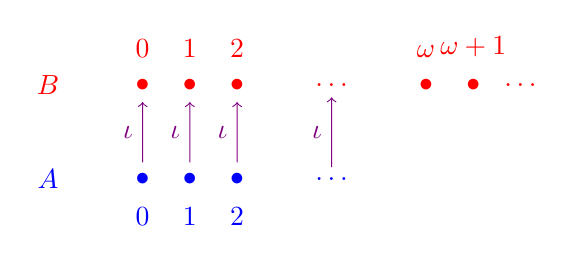
\begin{tikzpicture}[very thick, scale=0.6]
\begin{scope}[color=blue]
\node (A) at (0,0) {$A$};
\node(A0) at (2,0)[label=below:$0$]{$\bullet$};
\node(A1) at (3,0)[label=below:$1$]{$\bullet$};
\node(A2) at (4,0)[label=below:$2$]{$\bullet$};
\node (Adots) at (6,0) {$\ldots$};
\end{scope}
\begin{scope}[color=red]
\node (B) at (0,2) {$B$};
\node(B0) at (2,2)[label=above:$0$]{$\bullet$};
\node(B1) at (3,2)[label=above:$1$]{$\bullet$};
\node(B2) at (4,2)[label=above:$2$]{$\bullet$};
\node (Bdots) at (6,2) {$\ldots$};
\node (b) at (8,2) [label=above:$\omega$]{$\bullet$};
\node (bsucc) at (9,2) [label=above:$\omega+1$]{$\bullet$};
\node (Bdots2) at (10,2) {$\ldots$};
\end{scope}
\begin{scope}[color=red!50!blue]
\draw [->,thin] (A0) -- node [auto] {$\iota$} (B0);
\draw [->,thin] (A1) -- node [auto] {$\iota$} (B1);
\draw [->,thin] (A2) -- node [auto] {$\iota$} (B2);
\draw [->,thin] (Adots) -- node [auto] {$\iota$} (Bdots);
\end{scope}
\end{tikzpicture}
   \caption{\textcolor{blue}{$A$} is a sub-segment  of \textcolor{red}{$B$}}
   \label{fig:subsegment}
 \end{figure}

If \texttt{OB} is presumed to be correct, then we may consider that \texttt{OA} ``inherits'' its correctness from the bigger notation system \texttt{OB}.


\label{types:SubON}
\index{hydras}{Library OrdinalNotations!Type classes!SubON}

following definition
(in ~\href{../theories/html/hydras.OrdinalNotations.ON_Generic.html}{ON\_Generic}).

\input{movies/snippets/ON_Generic/SubONDef}



For instance, we prove that \texttt{Omega} is a sub-notation of
\texttt{Omega\_plus\_Omega} (with $\omega$ as the first ``new'' ordinal, and \texttt{fin} as the injection).

\vspace{10pt}

\noindent\emph{From Module~\href{../theories/html/hydras.OrdinalNotations.ON_Omega_plus_omega.html}{OrdinalNotations.ON\_Omega\_plus\_omega}}

\input{movies/snippets/ON_Omega_plus_omega/Incl}

We can also show that, if $i<j$, then the segment $[0,i)$ is a ``sub-segment'' of
$[0,j)$. Since the terms  ($t\;i$) and ($t\;j$) are not convertible, we consider a ``cast'' 
function $\iota$ from ($t\;i$) into ($t\;j$), and prove that this function is  a monotonous bijection  from ($t\;i$) to
the segment $[0,i)$ of ($t\;j$).

%\index{coq}{Commands!Program}

\vspace{10pt}

\noindent\emph{From Module~\href{../theories/html/hydras.OrdinalNotations.ON_Finite.html}{OrdinalNotations.ON\_Finite}}


\inputsnippets{ON_Finite/InclIJ, ON_Finite/InclIJa,
  ON_Finite/InclIJb,ON_Finite/InclIJc, ON_Finite/InclIJd,
ON_Finite/InclIJz}



\index{hydras}{Exercises}
\begin{exercise}
Prove that \texttt{Omega\_plus\_Omega} cannot be a sub-notation of \texttt{Omega}.
\end{exercise}

\index{hydras}{Projects}
\begin{project}
Adapt the definition of \texttt{Hvariant} (Sect.~\ref{sect:hvariant-def}) in order to
have an ordinal notation as argument. Prove that if $O_A$ is a sub-notation of $O_B$, then any variant defined on  $O_A$ can be automatically transformed into 
a variant on $O_B$.
\end{project}




\section{Comparing an ordinal notation with Schütte's model}

Finally, it may be interesting to compare an ordinal notation with the more theoretical model from Schütte (well, at least with our formalization of that model). This would be a relative proof of correctness of the considered  ordinal  notation.

The following class specifies that a notation \texttt{OA} describes a segment $[0,\alpha)$,
where $\alpha$ is a countable ordinal \emph{à la}  Schütte.


\label{types:ON-for}
\index{hydras}{Library OrdinalNotations!Type classes!ON\_correct}

\input{movies/snippets/ON_Generic/ONCorrect}


For instance, the following theorem tells that \texttt{Epsilon0}, our notation system for the segment $[0,\epsilon0)$ is a correct implementation of the theoretically defined  ordinal $\epsilon_0$
(see chapter~\ref{chap:schutte} for more details).

\vspace{4pt}
\noindent\emph{From Module~\href{../theories/html/hydras.Schutte.Correctness_E0.html}{Schutte.Correctness\_E0}}

\input{movies/snippets/Correctness_E0/Epsilon0Correct}



\index{hydras}{Projects}

\begin{project}
Same work, but replace Schütte's model with \gaia's.
\end{project}

\begin{project}
  When you have read Chapter~\ref{chap:schutte}, prove that the sum of two ordinal notations \texttt{ON\_plus} implements the addition of ordinals.
\end{project}





\section{Isomorphism of ordinal notations}


In some cases we want to show that two notation systems describe the same segment (for instance $[0,3+\omega)$ and $[0,\omega)$\;). For this purpose, one may prove that the two notation systems are order-isomorphic.

\index{hydras}{Library OrdinalNotations!Type classes!ON\_Iso}

\label{types:ON-iso} 


\input{movies/snippets/ON_Generic/ONIso}


\index{hydras}{Exercises}

\begin{exercise}
\label{exo:i-plus-omega}
Let $i$ be some natural number. Prove that the notation systems 
\texttt{Omega} and (\texttt{ON\_plus (OrdFin $i$) Omega}) are isomorphic.

{\it \textbf{Note:} This property reflects the equality $i+\omega=\omega$, that we prove also in larger notation systems, as well as in Schütte's model.}
This exercise is partially solved for $i=3$ (in ~\href{../theories/html/hydras.OrdinalNotations.Example_3PlusOmega.html}{OrdinalNotations.Example\_3PlusOmega}).

\end{exercise}

\index{hydras}{Projects}
\label{exo:ON-mult}
\begin{project}
% Define in \coq{} the product of two ordinal notations $N_A$ and $N_B$.
% If $A$ [resp. $B$] is the underlying type of $N_A$ [resp. $N_B$], the
% product \texttt{ON\_mult $N_A$ $N_B$} is implemented over the cartesian product $B\times A$ (with the lexicographic ordering).

This exercise is about the non-commutativity of the multiplication of ordinals, reflected in ordinal notations.

For instance, the
elements of the product (\texttt{ON\_mult Omega (FinOrd 3)}) are ordered as follows.
\[(0,0),(0,1),(0,2),(0,3),(0,4),\dots,{\color{red}(1,0),} (1,1),(1,2),\dots, {\color{red}(2,0)},(2,1),(2,2),\dots\]

Note that the elements of  (\texttt{ON\_mult (FinOrd 3) Omega}) are differently ordered (without limit ordinals):
\[(0,0),(1,0),(2,0),(0,1),(1,1),(2,1),(0,2),(1,2),(2,2),(0,3),\dots\]


Prove formally  that (\texttt{ON\_mult (FinOrd $i$) Omega}) is isomorphic to
\texttt{Omega}  whilst
\texttt{Omega}  is a sub-notation of (\texttt{ON\_mult Omega (FinOrd $i$)}),
for any strictly positive $i$. 

\textbf{Note:} Like Exercise~\ref{exo:i-plus-omega}, this project corresponds to the [in]equalities $i+\omega=\omega<\omega+i$, for any natural number $i$.
\end{project}

\index{hydras}{Projects}
\begin{project}
Consider two isomorphic ordinal notations \texttt{OA} and \texttt{OB}.
Prove that, if \texttt{OA} [resp. \texttt{OB}] is a correct implementation 
of $\alpha$ [resp. $\beta$], then $\alpha=\beta$.
\end{project}


\index{hydras}{Projects}
\begin{project}
\label{project:succ-limit-dec}
Add to the class \texttt{ON} the requirement that for any $\alpha$ it is decidable whether $\alpha$ is $0$, a successor or a limit ordinal.


\textbf{Hint:}   Beware of the instances associated with sum and product of notations!
  You may consider additional fields 
to make the sum and product of notations ``compositional''.

\end{project}

\index{hydras}{Projects}
\begin{project}
\label{project:on-setoid}
Reconsider the  class \texttt{ON}, with an equivalence instead of Leibniz equality.
\end{project}





%%%% ICI ICI

\section{Other ordinal notations}
%%% TODO : Fix the multiplication function in branch FixOmegaOmega

% \index{hydras}{Projects}

% \begin{project}
% The directory \texttt{theories/OmegaOmega} contains an ad-hoc formalization of $\omega^\omega$, contributed by Pascal Manoury. Every ordinal $\alpha$ is represented by a list $l$ whose elements are the coefficients of $\omega$ in  the Cantor normal form of $\alpha$ (in reverse order). For instance, the ordinal 
% $\omega^{8}\times 5 + \omega^{6}\times 8 + \omega^2\times 10 + \omega + 7$ is represented by the list \texttt{[5;0;8;0;0.0;10,1,7]}. 


%  Develop this representation and compare it with the other ordinal notations.



% \end{project}

\index{hydras}{Projects}

\begin{project}
Let $N_A$ be a notation system for ordinals strictly less than $\alpha$, 
with the strict order $(A,<_A)$. Please build the notation system
\texttt{ON\_Expl $N_A$}, on the type of multisets of elements of $A$
(or, if preferred, the type of non-increasing finite sequences on $A$,
provided with the lexicographic ordering on lists).

For instance, let us take $N_A=\texttt{Omega}$, and take $\alpha=\langle 4,4,2,1,0\rangle$,
 $\beta=\langle 4,3,3,3,3,3,2\rangle$, and $\gamma=\langle 5\rangle$. Then $\beta<\alpha<\gamma$. 

In contrast the list $\langle5,6,3,3\rangle$ is not non-increasing (\emph{i.e.} sorted w.r.t. $\geq$), so it is not to be considered.

Note that if the notation $N_A$ implements the ordinal 
$\alpha$,  the new notation $\omega^{N_A}$ must implement the ordinal $\phi_0(\alpha)$, a.k.a. $\omega^\alpha$ (see chapter~\ref{chap:schutte})

\end{project}



\begin{remark}
 The set of ordinal terms in Cantor normal form (see Chap.~\ref{chap:T1}) and 
in Veblen normal form (see 
\href{../theories/html/hydras.Gamma0.Gamma0.html}{Gamma0.Gamma0}) are shown to be ordinal notation systems, but there is a lot of work to be done in order to unify ad-hoc  definitions and proofs which were written before the definition of the \texttt{ON} type class.
\end{remark}

